\clearpage
\appendix

\crefalias{section}{appendix}
\crefalias{subsection}{appendix}

\begin{figure}[t]
\centering
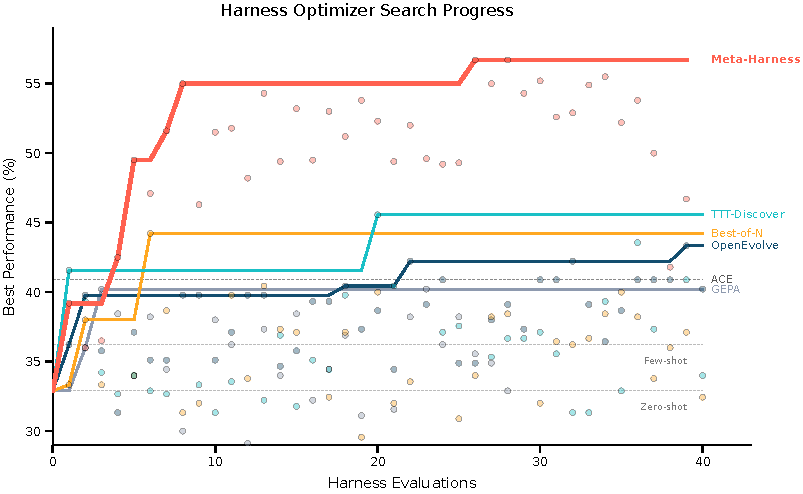
\includegraphics[width=0.99\linewidth]{figures/learning_curves.pdf}
\caption{
\label{fig:learning-curves-full}
Search-set accuracy over evaluations for all compared text optimizers on online text classification.
Each point is one candidate harness; lines track the best-so-far.
Per-dataset curves are shown alongside the aggregate.
\textbf{Meta-Harness reaches the final accuracy of OpenEvolve and TTT-Discover within the first 4 evaluations and continues improving, ending more than 10 points above all baselines.}
}
\end{figure}

\section{Qualitative Proposer Behavior}
\label{app:proposer-stats}

This section examines how the proposer uses the filesystem during search, drawing on the TerminalBench-2 run (10 iterations, \texttt{Claude Opus 4.6}).

\subsection{File Access Statistics}
\label{app:file-access-stats}

To verify that the proposer makes substantive use of the filesystem rather than defaulting to local edits, we recorded all file reads per iteration.

\Cref{tab:proposer-stats} summarizes the results.
The proposer reads a median of 82 files per iteration (range 69--99), roughly evenly split between prior harness source code (41\%) and execution traces (40\%), with the remainder going to score summaries (6\%) and other files (13\%).
This confirms that the proposer's access pattern is non-Markovian: it routinely inspects the majority of available history rather than conditioning only on the most recent parent.

\begin{table}[h]
\centering
\small
\begin{tabular}{@{}lr@{}}
\toprule
Statistic & Value \\
\midrule
Files read per iteration (median) & 82 \\
Files read per iteration (range) & 69--99 \\
\midrule
\multicolumn{2}{@{}l}{\textit{File type breakdown}} \\[2pt]
Harness source code & 41\% \\
Execution traces & 40\% \\
Score/summary files & 6\% \\
Other & 13\% \\
\bottomrule
\end{tabular}
\caption{Proposer file access statistics from the TerminalBench-2 search run (10 iterations, \texttt{Claude Opus 4.6}). The proposer reads extensively from the filesystem, with roughly equal attention to prior source code and execution traces.}
\label{tab:proposer-stats}
\end{table}

\subsection{Qualitative Behavior: Causal Reasoning Over Prior Failures}
\label{app:qualitative-behavior}

The TerminalBench-2 search log reveals a clear narrative arc in which the proposer learns from its own regressions.
Rather than wandering randomly through local edits, it forms an explicit diagnosis of why early candidates failed, then shifts toward a safer design pattern.
All text inside the log boxes below is quoted verbatim from the proposer's recorded reasoning at each iteration (emphasis ours).

\textbf{Iterations 1--2: promising bugfixes are confounded by prompt edits.}
The first two iterations both bundle plausible structural fixes with prompt-template modifications, and both regress sharply from the 64.4\% Terminus-KIRA baseline.
Iteration 1 targets observation corruption from leaked terminal markers and adds a loop breaker:

\begin{logbox}
Hypothesis: \_\_CMDEND\_\_ marker fragments leak into LLM observations on long-running tasks, causing the model to get confused and enter infinite no-tool-call loops. Stripping these markers + adding a loop breaker will recover wasted steps.
\end{logbox}

That candidate also introduced a new cleanup-oriented prompt template and a verification checklist.
Iteration 2 proposes a different state-machine fix:

\begin{logbox}
Double-confirmation completion mechanism causes verification spirals. Observed in trajectories where the agent solves the task early but burns 15--40+ additional steps re-verifying because each verification command resets \_pending\_completion, requiring another task\_complete $\rightarrow$ checklist $\rightarrow$ verify cycle.
\end{logbox}

This second candidate removes the pending-completion mechanism entirely, while also carrying over the marker stripping and the new prompt.
It still regresses, which gives the proposer two failed candidates with different structural changes but one shared prompt intervention.

\textbf{Iteration 3: the proposer identifies the confound.}
By iteration 3, the proposer explicitly infers that the regressions are not primarily due to the structural bugfixes themselves:

\begin{logbox}
Prior attempts: evo\_marker\_fix (58.9\%, -5.6pp), evo\_single\_confirm (57.8\%, -6.7pp) --- both regressed. \textbf{Root cause of regressions: Prompt template changes (cleanup directives) caused the agent to delete necessary state before task completion.} The structural bugfixes were confounded with harmful prompt changes. evo\_strip\_only isolates the two proven structural fixes.
\end{logbox}

This is the key causal step in the trajectory.
The proposer notices that the common factor across the first two failures is not the particular bugfix, but the cleanup-heavy prompt rewrite.
It therefore reverts to the original prompt and tests only the marker-stripping and loop-breaker.
The resulting candidate still underperforms slightly (63.3\%, -1.1pp), but it loses far less than the earlier versions, which supports the confound diagnosis.

\textbf{Iterations 4--6: direct fixes to the diagnosed failure mode still regress.}
The next three iterations continue to probe the same part of the design space, but now with more explicit theories about why the completion logic is fragile.
Iteration 4 attributes failures to a concrete state-machine bug in which verification commands reset the completion flag and trap the agent in repeated checklist cycles:

\begin{logbox}
Remove the two self.\_pending\_completion = False lines that reset the completion flag when intermediate commands run. This fixes a state machine bug where: (1) Agent calls task\_complete $\rightarrow$ sees QA checklist, \_pending\_completion = True (2) Agent runs verification commands $\rightarrow$ \_pending\_completion = False (bug!) (3) Agent calls task\_complete again $\rightarrow$ sees checklist AGAIN $\rightarrow$ infinite loop.
\end{logbox}

The proposer even cites concrete trajectory evidence, noting that \texttt{configure-git-webserver} produced baseline failures with agents stuck in 30--60 step verification spirals after effectively solving the task.
Iteration 5 tries to soften the cleanup language while preserving confirmation, but still edits the prompt and regresses badly.
Iteration 6 returns to the safer \texttt{evo\_strip\_only} base and proposes a systems-level optimization:

\begin{logbox}
Empty-command turns waste full LLM round-trips when terminal output hasn't changed. Smart-waiting (poll pane up to 3$\times$5s) before the next LLM call saves 5--15 turns on long-running tasks.
\end{logbox}

That change also regresses.
By this point, the proposer has learned a specific empirical lesson: modifications to prompts and completion flow are high risk, even when the local hypothesis sounds reasonable.

\textbf{Iteration 7: the winning candidate.}
After six consecutive regressions, the proposer shifts strategy from modifying the control loop to adding information before the loop begins:

\begin{logbox}
All 6 prior iterations regressed from the 64.4\% baseline because they modified the completion flow, prompt template, or observation processing. \textbf{evo\_env\_bootstrap takes a different approach --- purely additive.} It gathers an environment snapshot via a single shell command before the first LLM call and appends it to the initial prompt. No other methods are changed. This should eliminate 3--5 wasted exploration turns on dependency-heavy tasks without risking regression on already-passing tasks.
\end{logbox}

This candidate is the best result so far.
The important point is not just that iteration 7 wins, but that the proposer articulates \emph{why} it should be safer: it avoids touching the previously fragile completion machinery and instead adds information that is useful mainly on hard tasks.

\textbf{Iteration 8: composition.}
Having found one additive improvement, the proposer next attempts to compose it with an earlier structural fix:

\begin{logbox}
Combining two orthogonal fixes --- env snapshot (saves early exploration turns) + marker stripping with no-tool-call loop breaker --- will yield +1--3pp because they address independent failure modes without touching prompts or confirmation flows (which caused regressions in 5 of 7 prior iterations).
\end{logbox}

\textbf{Iteration 10: cross-run transfer.}
The proposer references results from a separate earlier search run:

\begin{logbox}
The evolution history showed ``don't cleanup service artifacts'' was worth +18pp. Iter 9 (evo\_no\_cleanup\_directive) targeted the same idea but crashed before evaluation.
\end{logbox}

\textbf{Summary.}
The search trajectory demonstrates that the proposer does more than random mutation.
Across the first seven iterations, it identifies a confound, tests the confound-isolating hypothesis directly, observes that control-flow and prompt edits remain fragile, and then deliberately pivots to a purely additive modification that becomes the best candidate in the run.
It subsequently tries to compose that winning idea with earlier fixes and even transfers lessons across runs.
This kind of causal reasoning over prior failures is precisely what full-history filesystem access enables and what compressed-feedback optimizers cannot support.


\section{Discovered Harnesses}
\label{app:discovered-harnesses}

Meta-Harness discovers executable inference-time procedures specific to the problem setup at hand.
These harnesses are structured, domain-specific policies, often with nontrivial control flow such as routing, filtering, and conditional context construction, selected solely by whether they improve search-set performance.
This section presents compact, method-style abstractions of representative harnesses that summarize the main behaviors and control-flow decisions that drive inference-time behavior.
For reference, the full implementation for each discovered harness is on the order of 100--1000 lines of code.

\subsection{Text Classification Harness}
\label{app:classification-harnesses}

In online text classification, Meta-Harness discovers a family of memory-based harnesses rather than a single canonical policy.
Table~\ref{tab:classification_pareto} reports the Pareto frontier of non-dominated variants from the main search, all selected solely by search-set performance.
We highlight two representative endpoints here: \ours{Meta-Harness (Draft Verification)}, the lowest-context frontier point, and \ours{Meta-Harness (Label-Primed Query)}, the highest-accuracy frontier point used in the main text.

\paragraph{Overview.}
Both harnesses maintain a growing memory of past labeled examples and build prompts from that memory at inference time.
What differs is the control flow used to interrogate the memory.
\ours{Meta-Harness (Draft Verification)} uses two short calls and explicitly tests the model's first guess against retrieved counterexamples, while \ours{Meta-Harness (Label-Primed Query)} spends a larger single-call budget on making the label space and local decision boundaries explicit.
\Cref{fig:classification-draft-verify,fig:classification-label-primed} summarize these two programs.

\paragraph{Meta-Harness (Draft Verification).}
The corresponding discovered file is \filename{draft_verification.py}.
This lightweight variant turns prediction into a two-call procedure.
It first retrieves the 5 most similar labeled examples and makes a draft prediction.
It then re-queries the same memory conditioned on that draft label, retrieving 5 \emph{confirmers} with the same label and 5 \emph{challengers} with different labels, and asks the model whether to maintain or revise its initial answer.
The key discovered behavior is that the second retrieval depends on both the query and the draft prediction, so the harness can surface counterexamples targeted at the model's current guess rather than only generic near neighbors.
If too few labeled examples have been accumulated, the program falls back to a standard single-call few-shot prompt.

\begin{figure}[t]
\centering
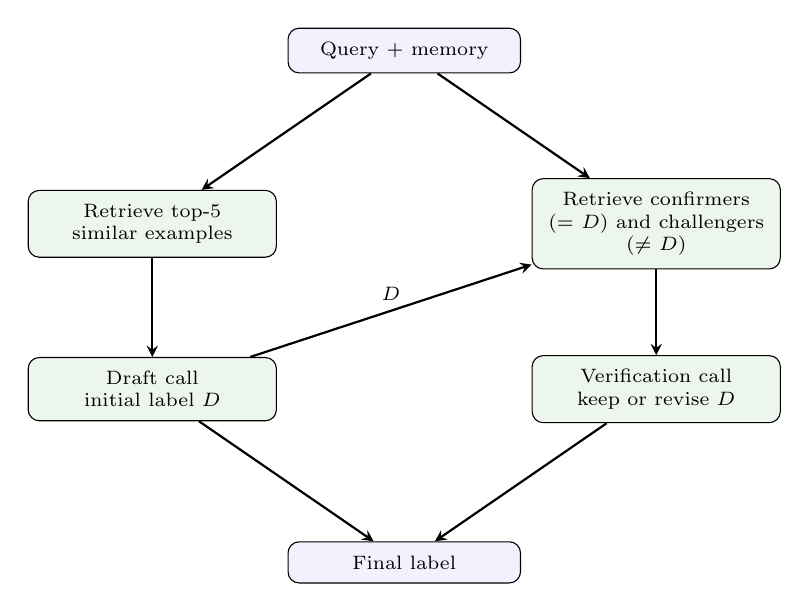
\begin{tikzpicture}[>=stealth, font=\scriptsize,
    box/.style={draw, rounded corners, align=center, fill=blue!5, inner sep=5pt, text width=2.6cm},
    stage/.style={draw, rounded corners, align=center, fill=ForestGreen!8, inner sep=5pt, text width=2.8cm}]
\node[box] (query) at (0, 0) {Query + memory};
\node[stage] (draftret) at (-3.2, -2.2) {Retrieve top-5\\ similar examples};
\node[stage] (draft) at (-3.2, -4.3) {Draft call\\ initial label $D$};
\node[stage] (verifyret) at (3.2, -2.2) {Retrieve confirmers\\ ($=$ $D$) and challengers\\ ($\neq$ $D$)};
\node[stage] (verify) at (3.2, -4.3) {Verification call\\ keep or revise $D$};
\node[box] (final) at (0, -6.5) {Final label};
\draw[->, thick] (query) -- (draftret);
\draw[->, thick] (draftret) -- (draft);
\draw[->, thick] (draft) -- node[above, font=\scriptsize] {$D$} (verifyret);
\draw[->, thick] (query) -- (verifyret);
\draw[->, thick] (verifyret) -- (verify);
\draw[->, thick] (draft) -- (final);
\draw[->, thick] (verify) -- (final);
\end{tikzpicture}
\caption{\textbf{Draft-verification classification harness.}
The first call produces a draft label from a short retrieved context.
The second call retrieves evidence for and against that draft and returns the final prediction.}
\label{fig:classification-draft-verify}
\end{figure}

\begin{itemize}[leftmargin=*]
\item \textbf{Stage 1: Draft.} Retrieve the 5 nearest labeled examples and ask for an initial prediction.
\item \textbf{Stage 2: Verification.} Condition retrieval on the draft label, then show both supporting and challenging examples before making the final prediction.
\item \textbf{Cold start.} If fewer than 5 labeled examples are available, skip the two-stage procedure and use a standard single-call few-shot prompt.
\item \textbf{Why it is cheap.} Both calls use short retrieved contexts, so the overall context cost stays near the low end of the frontier even with two model invocations.
\end{itemize}

\paragraph{Meta-Harness (Label-Primed Query).}
The corresponding discovered file is \filename{label_primed_query_anchored.py}.
This strongest variant uses a single larger call built from three parts.
It begins with a \emph{label primer} listing the valid output labels, then constructs a \emph{coverage} section with one query-relevant example per label, and finally adds \emph{query-anchored contrastive pairs} that place highly similar examples with different labels side by side.
The coverage block exposes the full label space, while the contrastive block sharpens local decision boundaries around the current query.
In code, the harness implements this with TF-IDF retrieval over past labeled examples and a query-anchored pairing rule that chooses contrasting examples from the same local neighborhood.

\begin{figure}[t]
\centering
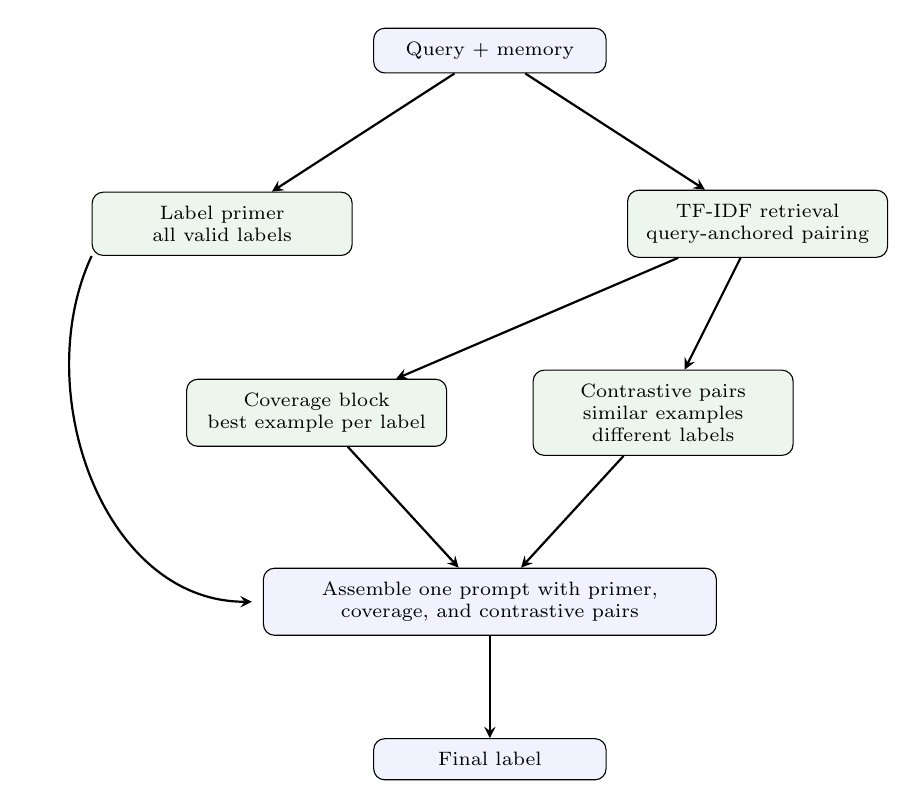
\begin{tikzpicture}[>=stealth, font=\scriptsize,
    box/.style={draw, rounded corners, align=center, fill=blue!5, inner sep=5pt, text width=2.6cm},
    stage/.style={draw, rounded corners, align=center, fill=ForestGreen!8, inner sep=5pt, text width=2.95cm}]
\node[box] (query) at (0, 0) {Query + memory};
\node[stage] (primer) at (-3.4, -2.2) {Label primer\\ all valid labels};
\node[stage] (retrieval) at (3.4, -2.2) {TF-IDF retrieval\\ query-anchored pairing};
\node[stage] (coverage) at (-2.2, -4.6) {Coverage block\\ best example per label};
\node[stage] (contrastive) at (2.2, -4.6) {Contrastive pairs\\ similar examples\\ different labels};
\node[box, text width=5.4cm] (prompt) at (0, -7.0) {Assemble one prompt with primer, coverage, and contrastive pairs};
\node[box] (final) at (0, -9.0) {Final label};
\draw[->, thick] (query) -- (primer);
\draw[->, thick] (query) -- (retrieval);
\draw[->, thick] (retrieval) -- (coverage);
\draw[->, thick] (retrieval) -- (contrastive);
\draw[->, thick] (primer.south west) to[out=-115,in=180] ([xshift=-4pt]prompt.west);
\draw[->, thick] (coverage) -- (prompt);
\draw[->, thick] (contrastive) -- (prompt);
\draw[->, thick] (prompt) -- (final);
\end{tikzpicture}
\caption{\textbf{Label-primed query-anchored classification harness.}
The program builds a single prompt that exposes the label space, then populates it with query-relevant coverage examples and local contrastive pairs.}
\label{fig:classification-label-primed}
\end{figure}

\begin{itemize}[leftmargin=*]
\item \textbf{Label primer.} List the valid output labels before showing any examples, so the model sees the full answer space up front.
\item \textbf{Coverage block.} For each known label, retrieve the most query-relevant labeled example and include one representative example per class.
\item \textbf{Contrastive block.} Build pairs of highly similar examples with different labels, so the prompt exposes local decision boundaries around the current query.
\item \textbf{Retrieval rule.} Use TF-IDF similarity and query-anchored partner selection rather than label-agnostic nearest neighbors.
\end{itemize}
\begin{table}[t]
\centering
\resizebox{\linewidth}{!}{
\begin{tabular}{
  l
  S[table-format=2.1, detect-weight]
  S[table-format=2.1, detect-weight]
  S[table-format=2.1, detect-weight]
  |
  S[table-format=2.1, detect-weight]
  S[table-format=2.1, detect-weight]
}
\toprule
& \multicolumn{3}{c|}{Datasets} & \multicolumn{2}{c}{Avg metrics} \\
\cmidrule(lr){2-4}\cmidrule(lr){5-6}
Variant & {USPTO $\uparrow$} & {Symptom $\uparrow$} & {LawBench $\uparrow$} & {Avg $\uparrow$} & {Ctx $\downarrow$} \\
\midrule
\ours{Meta-Harness (Draft Verification)} & {\bfseries 18.0} & 85.4 & 17.0 & 40.1 & 5.4 \\
\ours{Meta-Harness (Error-Annotated)} & 9.0 & 87.7 & 24.0 & 40.2 & 22.3 \\
\ours{Meta-Harness (CoT Replay)} & 13.0 & 88.2 & 25.0 & 42.1 & 23.3 \\
\ours{Meta-Harness (Cluster Coverage)} & 12.0 & 86.8 & 33.0 & 43.9 & 31.2 \\
\ours{Meta-Harness (Cascade Retrieval)} & 12.0 & 86.8 & 36.0 & 44.9 & 39.2 \\
\ours{Meta-Harness (RRF + Contrastive)} & {\bfseries 18.0} & 89.6 & 35.0 & 47.5 & 41.4 \\
\ours{Meta-Harness (Relevance + Contrastive)} & {\bfseries 18.0} & {\bfseries 90.6} & 36.0 & 48.2 & 43.9 \\
\ours{Meta-Harness (Label-Primed Query)} & 14.0 & 86.8 & {\bfseries 45.0} & {\bfseries 48.6} & 45.5 \\
\bottomrule
\end{tabular}
}
\caption{
    Pareto-optimal discovered variants from the main text-classification search, trading off average accuracy against context cost.
    The selected system in the main text is \ours{Meta-Harness (Label-Primed Query)}.
    Ctx denotes average additional characters in input context (thousands).
}
\label{tab:classification_pareto}
\end{table}


\begin{figure}[t]
\centering
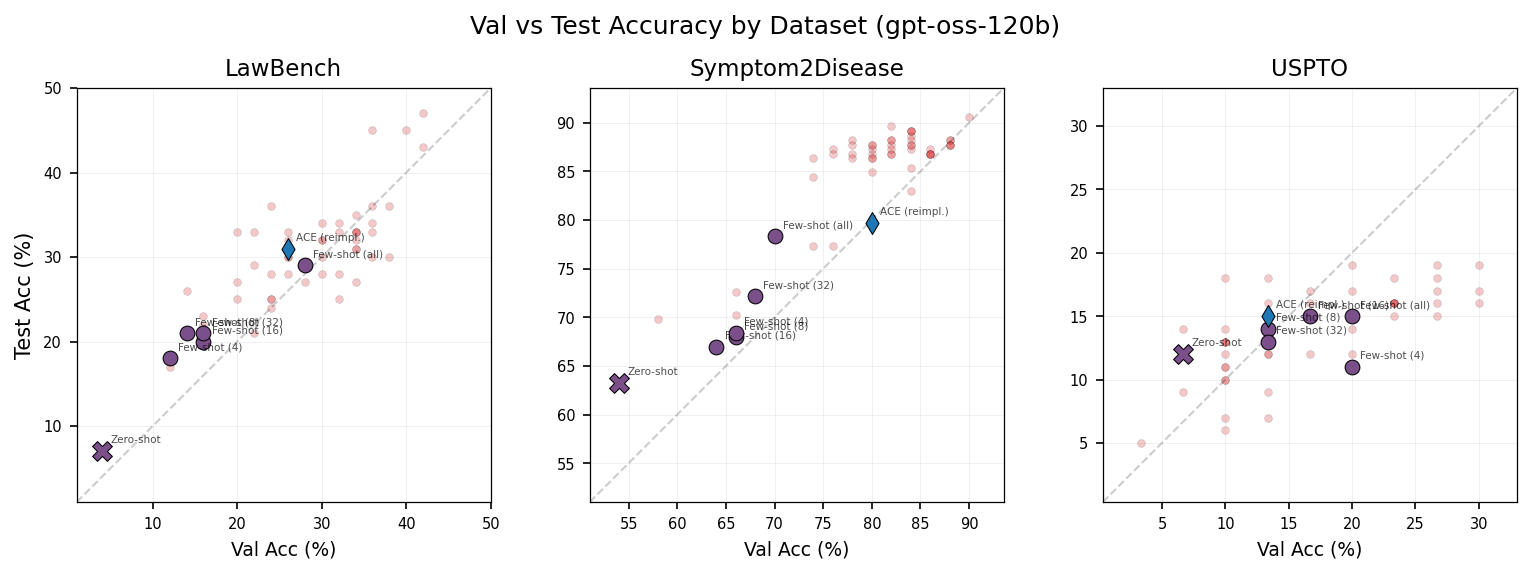
\includegraphics[width=\linewidth]{figures/val_vs_test_by_dataset.png}
\caption{Search-set vs.\ test accuracy per dataset for discovered text-classification strategies. Each pink dot is a discovered strategy; baselines are labeled. The dashed diagonal is $y{=}x$.}
\label{fig:val-vs-test}
\end{figure}

\subsection{Math Retrieval Harness}
\label{app:math-retriever}

This subsection describes the retrieval harness discovered by Meta-Harness for mathematical reasoning (\Cref{subsec:math-reasoning}).
The final harness is a compact four-route BM25 program whose structure emerged through search rather than being manually specified after the fact.
All design choices below---the routing predicates, reranking terms, deduplication thresholds, and per-route example counts---were selected by the outer loop across 40 iterations of evolution.

\paragraph{Overview.}
At inference time, the harness assigns each problem to exactly one of four routes: combinatorics, geometry, number theory, or a default route for algebra and other problems.
The gates are implemented as lightweight lexical predicates over the problem statement, including keyword sets and a small number of regex features for geometry notation.
The harness does not aggregate outputs across routes: once a route is selected, only that route retrieves examples for the final prompt.
All routes use BM25 as the underlying retrieval mechanism over the filtered corpus described above.
The BM25 index uses a math-aware tokenizer that preserves LaTeX tokens (e.g., \texttt{\textbackslash frac}, \texttt{\^{}\{2\}}) as atomic units.
The selected harness is a merge of two successful search lineages, autonomously combined by the proposer during search: one contributed a stronger geometry route based on raw BM25, while another contributed a stronger combinatorics route based on deduplication and difficulty reranking.
\Cref{fig:math-harness-diagram} gives a compact flowchart view of the final program.

\begin{figure}[t]
\centering
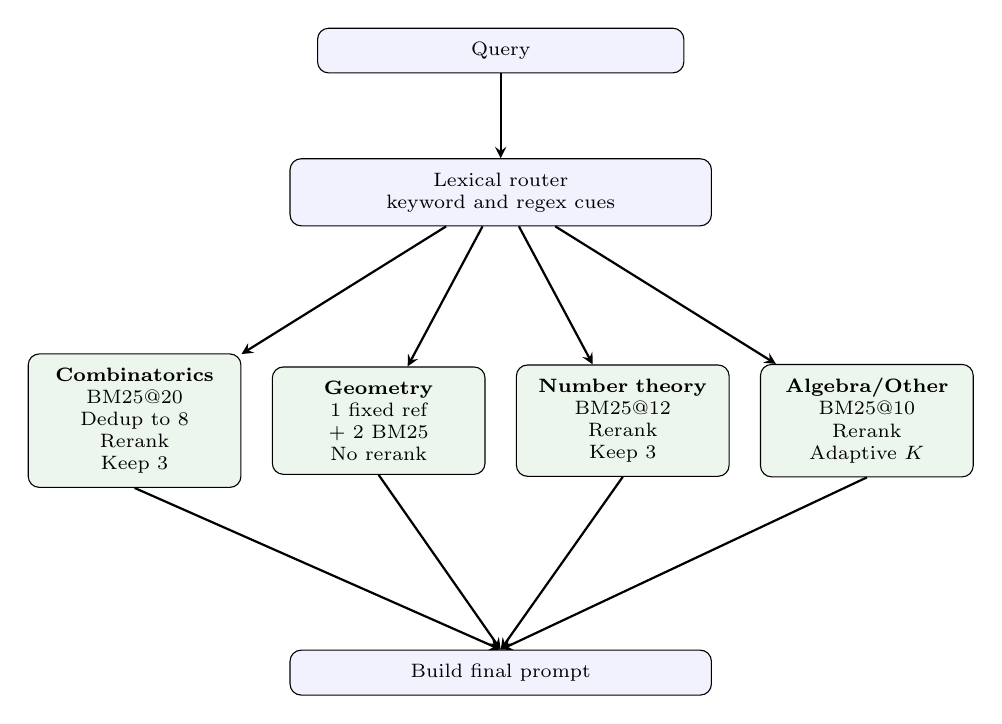
\begin{tikzpicture}[>=stealth, font=\scriptsize,
    box/.style={draw, rounded corners, align=center, fill=blue!5, inner sep=5pt, text width=4.3cm},
    route/.style={draw, rounded corners, align=center, fill=ForestGreen!8, inner sep=5pt, text width=2.35cm}]
\node[box] (query) at (0, 0) {Query};
\node[box, text width=5.0cm] (gate) at (0, -1.8) {Lexical router\\ keyword and regex cues};
\node[route] (comb) at (-4.65, -4.7) {\textbf{Combinatorics}\\ BM25@20\\ Dedup to 8\\ Rerank\\ Keep 3};
\node[route] (geo) at (-1.55, -4.7) {\textbf{Geometry}\\ 1 fixed ref + 2 BM25\\ No rerank};
\node[route] (nt) at (1.55, -4.7) {\textbf{Number theory}\\ BM25@12\\ Rerank\\ Keep 3};
\node[route] (rest) at (4.65, -4.7) {\textbf{Algebra/Other}\\ BM25@10\\ Rerank\\ Adaptive $K$};
\node[box, text width=5.0cm] (prompt) at (0, -7.9) {Build final prompt};
\draw[->, thick] (query) -- (gate);
\draw[->, thick] (gate) -- (comb);
\draw[->, thick] (gate) -- (geo);
\draw[->, thick] (gate) -- (nt);
\draw[->, thick] (gate) -- (rest);
\draw[->, thick] (comb.south) -- (prompt.north);
\draw[->, thick] (geo.south) -- (prompt.north);
\draw[->, thick] (nt.south) -- (prompt.north);
\draw[->, thick] (rest.south) -- (prompt.north);
\end{tikzpicture}
\caption{\textbf{Discovered math retrieval harness.}
A lexical router assigns each query to one of four subject-specific retrieval policies.
The selected policy retrieves examples, which are inserted into the final prompt.}
\label{fig:math-harness-diagram}
\end{figure}

\begin{itemize}[leftmargin=*]
\item \textbf{Combinatorics:} fetch 20 BM25 candidates, deduplicate to 8, rerank by lexical score and difficulty, then return the top 3. This is the main route where the harness explicitly trades off diversity against hard-problem matching.
\item \textbf{Geometry:} return 1 hard NuminaMath reference together with 2 raw BM25 neighbors. Search consistently prefers raw structural matches here over difficulty reranking.
\item \textbf{Number theory:} fetch 12 BM25 candidates and rerank using lexical score, difficulty, and a small bonus for solutions that state a technique early. This favors examples whose proof strategy is explicit.
\item \textbf{Default:} fetch 10 BM25 candidates, rerank by lexical score and difficulty, and choose an adaptive number of examples based on how concentrated the top retrieval scores are.
\end{itemize}

\subsection{TerminalBench-2 Harness}
\label{app:tbench-harness}

The discovered TerminalBench-2 harness builds on Terminus-KIRA~\citep{terminuskira2026}, inheriting its native tool calling (replacing Terminus~2's ICL-based JSON parsing), 30KB output cap, and multi-perspective completion checklist.
The main modification discovered by Meta-Harness is \textbf{environment bootstrapping}: before the agent loop begins, the harness runs a compound shell command to gather a snapshot of the sandbox environment and injects it into the initial prompt.
The proposer's hypothesis, recorded verbatim from the search log, was:

\begin{logbox}
Hypothesis: ``Injecting an environment snapshot (OS, installed languages, package managers, /app contents) before the first LLM turn will reduce wasted exploration episodes by 3--5 turns on dependency-heavy tasks''

Changes: ``Added \_gather\_env\_snapshot() that runs a single compound shell command to collect working directory, /app listing, available languages (python, gcc, node, java, rustc, go), package managers (pip, apt) [\ldots] and injects as [Environment Snapshot] block''
\end{logbox}

The snapshot includes: the working directory, a listing of \texttt{/app} (truncated to 20 entries for large directories), available programming languages and their versions (Python, GCC, G++, Node, Java, Rust, Go), installed package managers (pip, apt-get), and available memory.
This eliminates the 2--4 exploratory turns that agents typically spend discovering what tools and files are available, allowing the model to begin productive work immediately.
The bootstrapping command is guarded by a 15-second timeout and fails silently, so it does not break the agent in unusual environments.
The full implementation adds roughly 80 lines on top of Terminus-KIRA.
\Cref{fig:tbench-harness-diagram} summarizes the harness structure.

\paragraph{Per-task analysis.}
Compared to Terminus-KIRA, the discovered harness gains on 7 of 89 tasks, with the largest improvements on \texttt{protein-assembly} and \texttt{path-tracing}.
The gaining tasks share a common property: they require domain-specific tooling whose availability cannot be assumed in advance (bioinformatics libraries, rendering pipelines, chess engines, cryptographic utilities, CoreWars simulators).
Without the bootstrap, the agent spends its first 2--4 turns probing the environment; on tasks with tight turn budgets or where early wrong assumptions cascade, those wasted turns can be the difference between pass and fail.
This suggests that the bootstrap's value is largest when the environment is non-obvious, and the task requires the agent to match its strategy to what is actually installed.

\begin{figure}[t]
\centering
\begin{tikzpicture}[>=stealth, font=\scriptsize,
    box/.style={draw, rounded corners, align=center, fill=blue!5, inner sep=5pt, text width=3.2cm},
    stage/.style={draw, rounded corners, align=center, fill=ForestGreen!8, inner sep=5pt, text width=3.2cm},
    newstage/.style={draw, rounded corners, align=center, fill=ours-accent!15, inner sep=5pt, text width=3.2cm, draw=ours-accent}]
\node[box] (task) at (0, 0) {Task instruction};
\node[newstage] (bootstrap) at (0, -1.8) {\textbf{Env bootstrap}\\ pwd, files, languages,\\ pkg managers, memory};
\node[stage] (prompt) at (0, -3.8) {Initial prompt\\ task + snapshot};
\node[stage] (loop) at (0, -5.8) {Agent loop\\ native tool calling\\ 30KB output cap};
\node[stage] (check) at (0, -7.8) {Multi-perspective\\ completion checklist};
\node[box] (done) at (0, -9.6) {Task complete};
\draw[->, thick] (task) -- (bootstrap);
\draw[->, thick] (bootstrap) -- (prompt);
\draw[->, thick] (prompt) -- (loop);
\draw[->, thick] (loop) -- (check);
\draw[->, thick] (check) -- node[right, font=\scriptsize] {pass} (done);
\draw[->, thick] (check.east) to[out=0, in=0, looseness=1.5] node[right, font=\scriptsize] {fail} (loop.east);
\end{tikzpicture}
\caption{\textbf{Discovered TerminalBench-2 harness.}
The harness inherits Terminus-KIRA's native tool calling, output cap, and completion checklist (green).
The \colorbox{ours-accent!15}{environment bootstrap} (red) is the component discovered by Meta-Harness: it gathers a sandbox snapshot before the agent loop begins, eliminating early exploratory turns.}
\label{fig:tbench-harness-diagram}
\end{figure}

\section{Dataset Details}
\subsection{OOD Text Classification Datasets}
\label{app:text-classification-data}

\begin{itemize}[leftmargin=*,itemsep=2pt,topsep=2pt]
\item \textbf{SciCite} is a 3-way citation-intent classification benchmark introduced by \citet{cohan2019structuralscaffoldscitationintent}. Each example consists of a citation context from a scientific paper, labeled by the citation's rhetorical role, such as background, method, or result. The task tests whether a model can infer why one paper cites another from the local scientific context.
\item \textbf{FiNER-139} is a financial numeric entity recognition benchmark introduced by \citet{Loukas_2022}. It consists of word-level annotations from financial filings with 139 fine-grained XBRL entity types, making it substantially more fine-grained than standard sentence-level classification tasks. The benchmark tests whether a model can identify and classify numeric financial entities from context.
\item \textbf{Amazon Reviews} is the English portion of the Multilingual Amazon Reviews Corpus introduced by \citet{keung2020multilingualamazonreviewscorpus}. In our setting, it is used as a 5-way review rating prediction task, where the label corresponds to the review's star rating. This benchmark evaluates general-domain sentiment and rating prediction from product review text.
\item \textbf{Financial PhraseBank} is a 3-way financial sentiment benchmark introduced by \citet{malo2013gooddebtbaddebt}. It consists of sentences from financial news and related economic text labeled as positive, neutral, or negative with respect to market sentiment. The task evaluates domain-specific sentiment classification in finance.
\item \textbf{GoEmotions} is a fine-grained emotion classification benchmark introduced by \citet{demszky2020goemotionsdatasetfinegrainedemotions}. It contains English Reddit comments annotated with 27 emotion categories plus a neutral category, and is commonly treated as a 28-way classification task. The benchmark tests nuanced affect recognition beyond coarse positive-negative sentiment.
\item \textbf{Banking77} is a fine-grained intent classification benchmark introduced by \citet{casanueva2020efficientintentdetectiondual}. It contains online banking user utterances labeled with 77 intents, covering a wide range of customer service requests. The task evaluates single-domain intent detection with a large label space.
\item \textbf{AG News} is a 4-way news topic classification benchmark commonly associated with the text classification setup of \citet{zhang2016characterlevelconvolutionalnetworkstext}. Examples are labeled with broad news categories such as world, sports, business, and science/technology. It is a standard general-domain benchmark for topic classification.
\item \textbf{SciTail} is a science-domain textual entailment benchmark in which the task is to predict whether a hypothesis is entailed by a premise sentence in a science-focused inference setting~\citep{Khot_Sabharwal_Clark_2018}.
\item \textbf{TweetEval (Hate)} is the hate-speech subset of the TweetEval benchmark introduced by \citet{barbieri2020tweetevalunifiedbenchmarkcomparative}. It is a binary tweet classification task for detecting hateful versus non-hateful content within a unified social-media evaluation suite. This benchmark tests robust classification in noisy, short-form social media text.
\end{itemize}

\subsection{Math Retrieval Corpus}
\label{app:math-corpus}

\Cref{tab:math-corpus} lists the datasets composing the retrieval corpus used in \Cref{subsec:math-reasoning}.
The raw sources contain more problems than the final corpus; several filtering steps were applied before merging.
NuminaMath-1.5 was filtered to competition-math subsets (AMC/AIME, olympiad references, number theory, inequalities, and related sources), discarding lower-quality web-scraped entries.
OpenMathReasoning was deduplicated to one solution per problem (retaining the solution with the highest pass rate on an independent verifier), and problems whose source matched any evaluation benchmark family (IMO, AIME, HMMT, SMT, USAMO, Putnam) were removed before deduplication.
The entire corpus was then decontaminated against all evaluation benchmarks and the search set used during harness search, using exact prefix matching followed by fuzzy Jaccard similarity (threshold 0.8); any corpus problem matching an eval problem under either criterion was discarded.
Solutions from OpenMathReasoning and DeepMath are truncated to 5{,}000 characters to limit retrieval context length.
At runtime, the selected harness further restricts retrieval to entries with non-empty solutions shorter than 4{,}000 characters.
Retrieved solutions are truncated again to 3{,}000 characters when inserted into the prompt.
For the geometry route, the harness also constructs a separate hard-reference index from NuminaMath problems with difficulty greater than 6.

\begin{table}[h]
\centering
\begin{tabular}{lrrl}
\toprule
\textbf{Dataset} & \textbf{Problems} & \textbf{Sol. Len} & \textbf{Proof} \\
\midrule
\href{https://huggingface.co/datasets/nvidia/OpenMathReasoning}{OpenMathReasoning} & 281,743 & 5{,}000$^\dagger$ & 34\% \\
\href{https://huggingface.co/datasets/zwhe99/DeepMath-103K}{DeepMath-103K}     & 103,021 & 5{,}000$^\dagger$ & 0\%  \\
\href{https://huggingface.co/datasets/AI-MO/NuminaMath-1.5}{NuminaMath-1.5}    & 129,520 & 1{,}376           & 13\% \\
\href{https://huggingface.co/datasets/AIMO-Corpus/PolyMath}{PolyMath}          &  11,083 &     363           & 0\%  \\
\href{https://huggingface.co/datasets/KbsdJames/Omni-MATH}{Omni-MATH}         &   4,289 &     829           & 0\%  \\
\href{https://huggingface.co/datasets/SPIderman5/FineProofs-SFT}{FineProofs-SFT}    &   4,275 &   3{,}977         & 100\% \\
\href{https://huggingface.co/datasets/gneubig/aime-1983-2024}{AIME 1983--2024}   &     933 &     ---           & 0\%  \\
\href{https://huggingface.co/datasets/Putnam-AXIOM/putnam-axiom-dataset-v1}{Putnam-AXIOM}      &     492 &     888           & 100\% \\
\midrule
\textbf{Total}    & \textbf{535,356} & 5{,}000$^\dagger$ & 22\% \\
\bottomrule
\end{tabular}

\smallskip
{\footnotesize $^\dagger$ Truncated at 5{,}000 characters; actual solutions are longer.}
\caption{
    Datasets in the math retrieval corpus (535K problems total).
    Sol. \ Len is the median solution length in characters.
    Proof indicates whether the dataset contains proof-type problems (by answer or problem type field).}
\label{tab:math-corpus}
\end{table}

\subsection{Math IMO-level Test Set}
\label{app:math-per-dataset}

The main text aggregates results over 200 IMO-level problems drawn from IMO-AnswerBench, IMO-ProofBench, ArXivMath December 2025, and ArXivMath January 2026.
The 200-problem evaluation set consists of a stratified 100-problem subset of IMO-AnswerBench, together with all problems from the other three benchmarks.
This per-benchmark breakdown is useful because the four datasets mix answer-style, proof, and research-style problems, which are aggregated together in the main paper for brevity.
When included, the table in this section should report each benchmark separately for both \texttt{Base} and \texttt{Meta-Harness} across the five held-out models.

\begin{table}[h]
\centering
\begin{tabular}{lr}
\toprule
\textbf{Dataset} & \textbf{Problems} \\
\midrule
IMO-AnswerBench & 100 \\
IMO-ProofBench & 60 \\
ArXivMath Dec.\ 2025 & 17 \\
ArXivMath Jan.\ 2026 & 23 \\
\midrule
\textbf{Total} & \textbf{200} \\
\bottomrule
\end{tabular}
\caption{
    Breakdown of the 200-problem IMO-level evaluation set.}
\label{tab:math_eval_breakdown}
\end{table}


\section{Practical Implementation Tips}
\label{app:practical-tips}

Meta-Harness is largely domain-agnostic: we expect it to apply in any setting where a language model is wrapped by a task-specific harness.
Applying it in a new domain, however, requires operating in a relatively new regime of LLM-assisted coding, where the proposer conditions on long-horizon histories of prior runs and writes programs whose effects may only become visible many steps later.
In getting this workflow to work reliably, we found a small set of practical choices that mattered consistently across the three domains studied in this paper.
The guidelines below are not themselves scientific claims about the method; they are engineering lessons from building and running the system, which we hope will make it easier for future work to apply Meta-Harness in other domains.

\begin{itemize}[leftmargin=*]

\item \textbf{Write a good skill.}
The skill text is the primary interface for steering the search, and its quality is the strongest lever on whether the loop works.
The proposer receives a natural-language skill~\citep{agentskills} that defines its role, the directory layout, CLI commands, and output format.
In practice, the skill should constrain outputs and safety-relevant behavior, not the proposer's diagnosis procedure: it should specify what is forbidden, what artifacts to produce, and what objectives to optimize, while leaving the model free to inspect scores, traces, and prior code as needed.
Our intuition from inspecting logs from Meta-Harness runs is that after enough iterations, the accumulated traces often shape the proposer's behavior more than the skill itself.
In our experience, iterating on the skill text had a larger effect on search quality than changing iteration count or population size.
Expect to run a few short evolution runs (3--5 iterations each) specifically to debug and refine the skill before committing to a full run.

\item \textbf{Start with a baseline harness and a search set that is hard for it.}
Write a simple baseline (e.g., few-shot prompting), then construct the search set by either filtering for examples that the baseline gets wrong or selecting a diverse subset of difficult instances.
The search has little to optimize if the baseline already saturates the evaluation.
Keep the search set small enough for roughly 50 full evaluations per run (50--100 examples in our classification experiments, 88 problems for math retrieval); a fast, discriminative eval is more valuable than a large one.

\item \textbf{Log everything in a format that is easy to navigate.}
Evaluation code should write code, scores, and execution traces in a form that the proposer can query reliably.
In practice, this means using machine-readable formats such as JSON, organizing artifacts hierarchically, choosing reasonable and consistent file names, and adopting naming schemes that make simple tools such as regex search work well.

\item \textbf{Make logs queryable through a small CLI (optional, but helpful).}
Each harness gets a directory containing source code, scores, and execution traces, but as the history grows, raw filesystem access alone becomes cumbersome.
A short CLI that lists the Pareto frontier, shows top-$k$ harnesses, and diffs code and results between pairs of runs can make the experience store much easier to use, and querying such CLIs is closely aligned with the workflows on which coding agents are trained.
If relevant offline experience exists (rollouts from other models, solved problem corpora, relevant papers), converting it into the same directory structure can also help warm-start exploration and ground new ideas.
This layer helps the proposer save tokens it may have wasted on navigation.

\item \textbf{Lightweight validation before expensive benchmarks.}
Write a small validation test that imports the module, instantiates the class, and calls both methods on a tiny set of examples.
Harnesses proposed during the search should pass this test before being fully evaluated.
A simple test script can catch most malformed or nonfunctional candidates in seconds and keep the cost of failures near zero.

\item \textbf{Automate evaluation outside the proposer.}
Running evals is simple enough that it is not worth making the proposer do it.
A separate harness should score candidates and write results to the filesystem.

\end{itemize}

\section{Extended Related Work}
\label{app:extended-related-work}

This appendix expands the brief discussion in \Cref{sec:related-work} and situates Meta-Harness relative to several neighboring lines of work that we could not cover in detail in the main text. A recurring distinction is that Meta-
Harness optimizes executable harness implementations and provides the proposer with selective access to prior code, scores, and execution traces via the filesystem.

\paragraph{AlphaEvolve / OpenEvolve.}
AlphaEvolve~\citep{novikov2025alphaevolve} and OpenEvolve~\citep{openevolve} evolve code via LLM-guided mutations with structured feedback: the proposer receives a program database with scalar scores (4--22K tokens per step; \Cref{tab:task_comparison}) and applies fixed mutation strategies to tournament-selected parents.
These methods are designed for algorithm discovery and optimization (mathematical conjectures, scheduling heuristics, hardware kernels), where the search target is a single stateless function with a clean scalar objective, and mutations are local.
Harness engineering is a different regime: harnesses are stateful programs that accumulate experience across many examples, and a single design choice (e.g., what to store in memory) can cascade through an entire evaluation sequence.
Meta-Harness addresses this by giving an unstructured coding agent full filesystem access, letting it selectively read any prior candidate's source code, execution traces, and scores.

\paragraph{GEPA.}
GEPA~\citep{agrawal2025gepa} is the closest text optimizer in terms of feedback richness, providing rollout traces per candidate.
It is designed for prompt optimization on tasks with short feedback loops (math problems, instruction-following, code optimization), where each rollout is a single LLM call or a short pipeline.
In this regime, per-candidate reflection works well: one prompt, one answer, one score.
Harness engineering requires reasoning across many examples and many candidates simultaneously: understanding why a retrieval strategy works for one class of problems but degrades on another requires comparing execution traces across the full population.
GEPA operates on one candidate at a time (2--8K tokens per step; \Cref{tab:task_comparison}), with a fixed critique format that must anticipate what information is relevant.
Meta-Harness gives the proposer access to \textit{all} prior candidates simultaneously and lets the agent decide what to examine.

\paragraph{Prompt orchestration frameworks.}
Several systems provide structured abstractions for composing multi-stage LLM programs. LMQL~\citep{Beurer_Kellner_2023}, LangChain~\citep{chase2022langchain}, and DSPy~\citep{khattab2023dspycompilingdeclarativelanguage} make prompt engineering more systematic by providing higher-level interfaces for prompt templates, control flow, and modular LLM pipelines. These frameworks help developers specify and organize LLM programs, but they still typically require manual design of retrieval policies, memory updates, and orchestration logic. Meta-Harness operates at a different level: it searches over the \emph{implementation} of these policies in executable code, treating the harness itself as the optimization target.
